\documentclass[tikz,border=3pt]{standalone}
\usepackage{xcolor}
\usetikzlibrary{arrows.meta,decorations.pathreplacing,positioning}
\definecolor{flowblue}{HTML}{2563EB}
\definecolor{flowgray}{HTML}{475569}
\definecolor{flowfill}{HTML}{F1F5F9}
\begin{document}
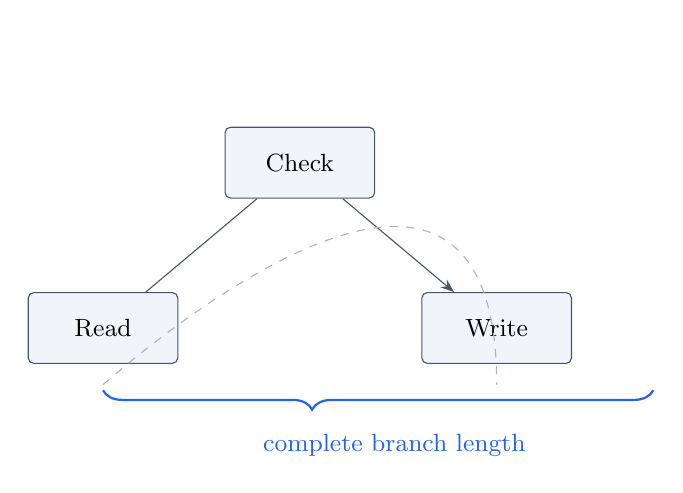
\begin{tikzpicture}[
  >=Stealth,
  stage/.style={draw=flowgray,fill=flowfill,rounded corners=2pt,
    minimum width=19mm,minimum height=9mm},
  every node/.style={font=\small}
]
  \node[stage] (read) at (0,0) {Read};
  \node[stage] (check) at (2.5,2.1) {Check};
  \node[stage] (write) at (5,0) {Write};
  \draw[flowgray,-Stealth] (read) -- (check) -- (write);
  \draw[flowgray!45,dashed]
    (0,-.72) .. controls (.01,-.72) and (5,3.8) .. (5,-.72);
  \draw[flowblue,line width=.8pt,decorate,
    decoration={brace,amplitude=7pt,aspect=.38,mirror,raise=2pt}]
    (0,-.72) .. controls (.01,-.72) and (5,3.8) .. (5,-.72);
  \node[flowblue,below] at (3.7,-1.22) {complete branch length};
\end{tikzpicture}
\end{document}
